\chapter{Code Structure and Input\\ Parameters} \label{ch:source code struct}
This section describes the WEC-Sim source code and the code structure. For the purposes of this document, we define the the source code as the MATLAB m-files that read the user input data, perform pre-processing calculations that take place before the Simulink/SimMechanics time-domain simulations are performed.

\section{Units}
All units within WEC-Sim are in the MKS (meters-kilograms-seconds system) and angular measurements are specified in radians unless otherwise specified.

\section{WEC-Sim Input File}
A WEC-Sim input file is required for each run. It MUST be placed inside the case directory for the run and MUST be named \texttt{wecSimInputFile.m}.  Figure~\ref{fig:inputFile} shows an example of the input file for a two-body point absorber. The input file contains information needed to run WEC-Sim simulations. Specifically, it serves four primary functions, each of which will be described in the following paragraphs.

\subsection{Specification of Simulation Parameters}
Within the input file, the user specifies simulation parameters, such as simulation duration and time step. As shown in Figure~\ref{fig:inputFile}, simulation parameters are specified within the \texttt{simu} variable, which is a member of the \texttt{simulationClass}. Users also specify the name of the Simulink/SimMechanics WEC model within the \texttt{simu} variable. The simulation parameters that are available for the user to set within the \texttt{simulationClass} are described in more detail in Section~\ref{subsec:simulationClass}.

\subsection{Specification of Body Parameters}
WEC-Sim assumes that every WEC devices is composed of rigid bodies that are exposed to wave forces. For each body, users MUST specify body properties within the \texttt{body} variable in the input file, including mass, moment of inertia, center of gravity, and the WAMIT files that describe the hydrodynamic properties (see Figure~\ref{fig:inputFile}). The body parameters that are available for the user to set within the \texttt{bodyClass} are described in more detail in Section~\ref{subsec:bodyClass}.

\begin{figure}[H]
\centering
\lstinputlisting{application/images/RM3wecSimInputFile.m}
\caption{Example of a WEC-Sim input file (same to Figure~\ref{fig:RM3inputFile}).}
\label{fig:inputFile}
\end{figure}

\subsection{Specification of Wave Parameters}
Within the input file,  users MUST provide information on the wave condition for the simulation. The user MUST specify the wave condition within the \texttt{waves} variable. The options that are available for the user to set within the \texttt{waveClass} are discussed in more detail in Section~\ref{subsec:waveClass}.

\subsection{Specification of Power Take-Off and Constraint Parameters}
PTO and constraint blocks connect WEC bodies to each other (and possibly to the seabed). The properties of the PTO and constraint are defined within \texttt{pto} variable and \texttt{constraint} variable, respectively. The options that are available for the user to specify are described in more detail in Sections \ref{subsec:constraint} and \ref{subsec:pto} .

\section{WEC-Sim Code}\label{sec:wecSimCode}
All data that are needed for a WEC-Sim simulation are contained within \texttt{simu}, \texttt{body}, \texttt{waves}, \texttt{pto} and \texttt{constraint} variables that are instances of the \texttt{simulationClass}, \texttt{bodyClass}, \texttt{wavesClass}, and \texttt{jointClass} objects, respectively. These objects are created in  \href{http://www.mathworks.com/help/matlab/matlab_oop/classes-in-the-matlab-language.html}{MATLAB classes}. The user can interact with these variables within the WEC-Sim input file, \texttt{wecSimInputFile.m}, (see Figure~\ref{fig:inputFile}). The remainder of this section describes the data within the WEC-Sim objects and how to interact with the objects to set relevant simulation input parameters. Examples of using WEC-Sim to simulate WEC devices and input files are described in \hyperlink{chapter.6}{Chapter 6}.

\subsection{\texttt{simulationClass}}\label{subsec:simulationClass}
The \texttt{simulationClass} contains the simulation parameters and solver settings needed to execute WEC-Sim. The user can set the relevant simulation properties in the \texttt{wecSimInputFile.m}. The user MUST specify the name of the Simulink/SimMechanics WEC model, which can be set by entering the following command in the input file

\begin{center}\texttt{\qquad{}simu.simMechanicsFile='<WEC Model Name>.slx';}\end{center}

By doing nothing, users have the option of accepting the default values for all the other simulation parameters. Available simulation properties and the default values for each, shown in Figure~\ref{fig:simulationClass}, can be explored further by typing \texttt{doc simulationClass} from within the MATLAB Command Window. The users can also specify simulation parameters and solver settings  in the input file to overwrite the default values. For example, the end time of a simulation can be set by entering the following command

\begin{center}\texttt{simu.endTime = <user specified end time>}\end{center}

\begin{figure}[H]
\centering
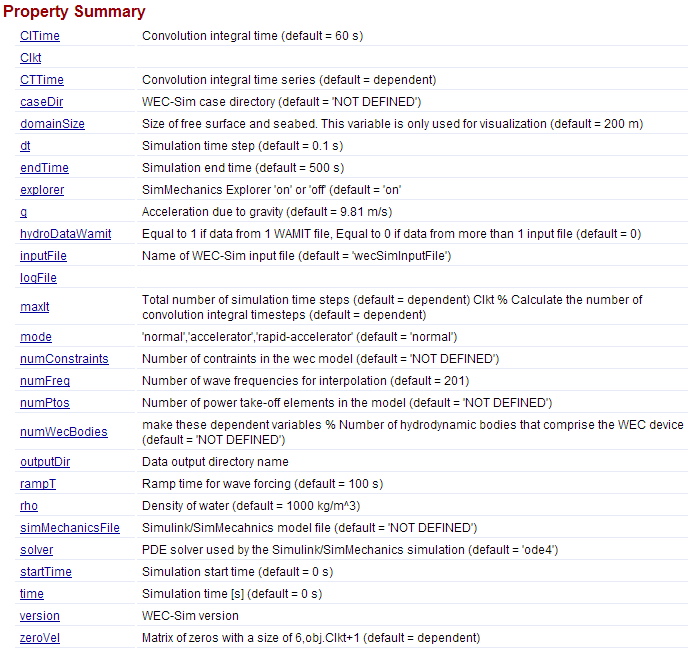
\includegraphics[width=1\textwidth]{codeStruct/images/simulationClass}
\caption{Data contained within the \texttt{simulationClass.}}
\label{fig:simulationClass}
\end{figure}

\subsection{\texttt{bodyClass}}\label{subsec:bodyClass}

The \texttt{bodyClass} object contains the mass and hydrodynamic properties of each body that comprises the WEC device being simulated. Each body must have a \texttt{bodyClass} initiated in the input file. we recommend that these body objects be named \texttt{body(<body number>)} as shown in the input file in Figure~\ref{fig:inputFile}. Each body object MUST be initiated by entering the command

\begin{center}\texttt{\qquad{}body(<body number>)=bodyClass('<body name>'),}\end{center}

Users can specify the mass and hydrodynamic properties after the body object is initiated for each body. Note that the \texttt{hydroDataType}, \texttt{hydroDataLocation}, \texttt{mass}, \texttt{cg}, \texttt{momOfInertia} and \texttt{geometry} parameters all have to be specified for each body as shown in Figure~\ref{fig:inputFile}. 

The users have the option of accepting the default values for the remaining body parameters by doing nothing or specify their own values. The options available within the \texttt{bodyClass} are shown in Figure~\ref{fig:bodyClass}. For example, the viscous drag can be specified by entering the viscous drag coefficient (nondimensional) and the projected characteristic area (in ${m^2}$) in vector format the input file as follows,

\begin{center}\texttt{\qquad{}body(<body number>).cd= [0 0 1.3 0 0 0],}\end{center}
\begin{center}\texttt{\qquad{}body(<body number>).characteristicArea= [0 0 100 0 0 0],}\end{center}

\begin{figure}[H]
\centering
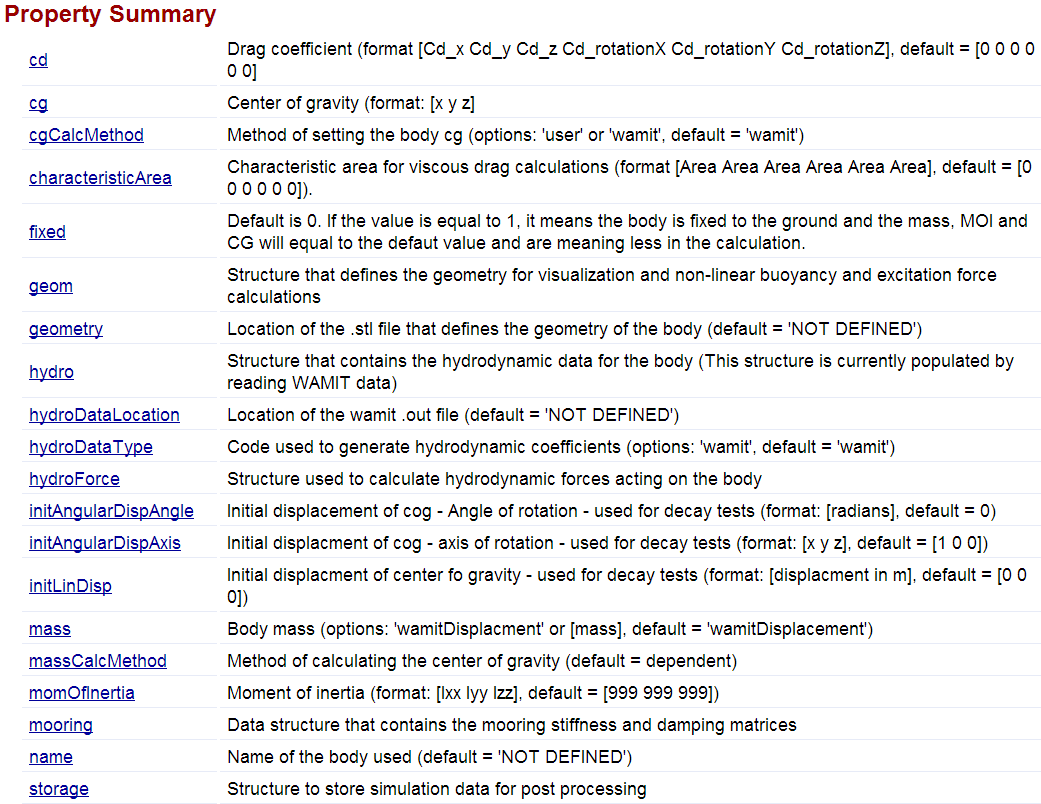
\includegraphics[width=1\textwidth]{codeStruct/images/bodyClass}
\caption{Data contained within the \texttt{bodyClass}.}
\label{fig:bodyClass}
\end{figure}
\clearpage
\subsection{\texttt{waveClass}}\label{subsec:waveClass}
The \texttt{waveClass} contains all the information that defines the wave conditions for the time-domain simulation. Specifically, Table~\ref{Table: List of supported wave environments} lists the types of wave environment that is supported by WEC-Sim.

\begin{table}[H]
\noindent \centering{}\protect\caption{List of supported wave environments}
\begin{tabular}{|c|c|c|}
\hline 
 \textbf{Option} & \textbf{Additional required inputs}  & \textbf{Description} \tabularnewline
\hline 
waves.type&  &Free decay test with\\
='noWave'&waves.noWaveHydrodynamicCoeffT&constant hydrodynamic coefficients\tabularnewline
\hline 
waves.type& & Free decay test with\\
='noWaveCIC'&None&convolution integral\tabularnewline
\hline 
waves.type &waves.H; &Sinusoidal steady-state\\
='regular'&waves.T &Reponse Scenario\tabularnewline
\hline 
waves.type &waves.H; &Regular waves with\\
='regularCIC'&waves.T &convolution integral\tabularnewline
\hline 
waves.type&waves.H; waves.T; &Irregular waves with\\
='irregular'&waves.spectrumType&typical wave spectrum\tabularnewline
\hline 
waves.type&&Irregular waves with\\
='irregularImport'&waves.spectrumDataFile&user-defined wave spectrum\tabularnewline
\hline 
\end{tabular}
\label{Table: List of supported wave environments}
\end{table}
\begin{itemize}
\item \textbf{No waves (\texttt{waves.type='noWave'})}: It is the wave type for running simulations without waves and using constant added mass and radiation damping coefficients. Accordingly, the user must still run WAMIT before executing WEC-Sim. In addition, users MUST specify the period from which the hydrodynamic coefficients are selected by setting the \texttt{waves.noWaveHydrodynamicCoeffT} variable. This option is typically used for decay tests for comparison with analytical solutions that use given radiation added-mass and damping coefficients.

\item \textbf{No waves with convolution integral calculation (\texttt{waves.type='noWaveCIC'})}: The wave type is the same as \texttt{noWave}, except the radiation forces are calculated using the convolution integral and the infinite frequency added mass .

\item \textbf{Regular waves (\texttt{waves.type='regular'})}: It is the wave type for running simulations using regular waves with constant added mass and radiation damping coefficients. Wave period \texttt{wave.T} and wave height \texttt{wave.H} need to be specified in the input file. Using this option, we assume that the system dynamic response is in sinusoidal steady-state form, where constant added mass and damping coefficients are used and the convolution integral is NOT used to calculate wave radiation forces.

\item \textbf{Regular waves with convolution integral (\texttt{waves.type='regularCIC'})}: The wave type is the same as \texttt{waves.type='regular'}, except the radiation forces are calculated using the convolution integral and the infinite frequency added mass.
\clearpage
\item \textbf{Irregular waves (\texttt{waves.type='irregular'})}: It is the wave type for irregular wave simulations using given wave spectrum. Significant wave height \texttt{wave.H}, peak period \texttt{wave.T} and  wave spectrum type (\texttt{waves.spectrumtype}) need to be specified in the input file. The available wave spectrum options are listed in Table~\ref{Table: Available wave spectrum options}.

\begin{table}[H]
\noindent \centering{}\protect\caption{WEC-Sim wave spectrum options (with \texttt{waves.type='irregular'})}
\begin{tabular}{|c|c|c|}
\hline 
\textbf{Wave Spectrum Type}  & \textbf{Input File Parameter} \tabularnewline
\hline 
Pierson--Moskowitz &\texttt{waves.spectrumType='PM'}\tabularnewline
\hline 
Bretschneider &\texttt{waves.spectrumType='BS'}\tabularnewline
\hline 
JONSWAP &\texttt{waves.spectrumType='JS'}\tabularnewline
\hline 
\end{tabular}
\label{Table: Available wave spectrum options}
\end{table}

\item \textbf{Irregular waves with user-defined spectrum (\texttt{waves.type='irregularImport'})}:  It is the wave type for irregular wave simulations using user-defined wave spectrum. Users need to specify the wave spectrum file name in input file as follows,

\begin{center}\texttt{\qquad{}waves.spectrumDataFile='<wave spectrum file>.txt',}\end{center}

The user-defined wave spectrum must be defined with the wave frequency (Hz) in the first row, and the spectral energy density $\frac{m^2}{Hz}$ in the second row. An example of which is given in the \texttt{ndbcBuoyData.txt} file in the applications folder of the WEC-Sim download. This format can be copied directly from NDBC buoy data. For more information on NDBC buoy data measurement descriptions, please refer to NDBC website at \href{http://www.ndbc.noaa.gov/measdes.shtml}{http://www.ndbc.noaa.gov/measdes.shtml}.\\
\end{itemize}

Note that, by default, the random wave phase for irregular waves are generated arbitrarily (\texttt{waves.randPreDefined=0}). If the user specifies \texttt{waves.randPreDefined=1} in the input file, the random phase of the waves will be generated using the \texttt{rand} function in MATLAB with a seed value of  1. This gives the user an option to generate the same random wave every time if needed. 

Typing \texttt{doc waveClass} from the MATLAB Command Window provides more information on the class functionality and the available wave properties are shown and described in Figure~\ref{fig:waveClass}.

\begin{figure}[h]
\centering
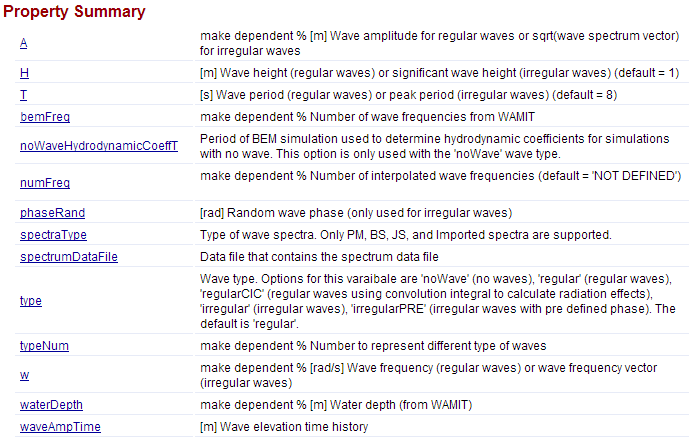
\includegraphics[width=1\textwidth]{codeStruct/images/waveClass}
\caption{Data contained within the \texttt{waveClass.}}
\label{fig:waveClass}
\end{figure}

\subsection{\texttt{constraintClass}}\label{subsec:constraint}
The constraint object is used to connect bodies to the Global Reference Frame. The constraint variable should be initiated by entering the following:

\begin{center}\texttt{constraint(<constraint number>)=constraintClass('<constraint name>');}\end{center} 

For rotational constraint (i.e., pitch), the user also needs to specify its location of the rotational joint with respect to the global reference frame in the \texttt{constraint(<constraint number>).loc} variable.

\subsection{\texttt{ptoClass}}\label{subsec:pto}
The pto object extracts power from body motion with respect to a fixed reference frame or another body. The pto objects can also constrain motion to certain degrees of freedom. The pto variable should be initiated by entering

\begin{center}\texttt{pto(<pto number>)=ptoClass('<pto name>'),}\end{center} 

For rotational ptos (Local RY), the user also needs to set its location. The users also have the option to specify the damping (\texttt{pto(<pto number>).c}) and stiffness (\texttt{pto(<pto number>).k}) values to represent the PTO system. Both have a default value of 0, and the users can overwrite the default values in the input file. For example, the users can specify a damping value by entering the following:

\begin{center}\texttt{pto(<pto number>).c=<pto damping value>,}\end{center}.

